\documentclass[10pt,mathserif,aspectratio=169]{beamer}

\usepackage{graphicx,amsmath,amssymb,tikz,psfrag,booktabs}

% \renewcommand{\familydefault}{\sfdefault}
\newcommand{\indep}{\perp\!\!\!\!\perp} % the independent symbol

% define theorem
\newtheorem{theorem}{Theorem}[section]
\newtheorem{corollary}[theorem]{Corollary}
\newtheorem{assumption}{Assumption}[subsection]
% define definition style
\theoremstyle{definition}
\newtheorem{definition}{Definition}[section]
\newtheorem{proposition}{Proposition}[section]
\newtheorem{property}{Property}[section]
\newtheorem{example}{Example}[section]
\newtheorem*{exercise}{Exercise}
% define remark style
\theoremstyle{remark}
\newtheorem*{remark}{Remark}
\newtheorem{question}{Question}

\newcommand{\R}{\mathbb{R}}
\newcommand{\C}{\mathbb{C}}
\newcommand{\Rd}{\mathbb{R}^d}
\newcommand{\Hy}{\mathbb{H}}
\newcommand{\calh}{\mathcal{H}}
\newcommand{\cala}{\mathcal{A}}
\newcommand{\calm}{\mathcal{M}}
\newcommand{\cald}{\mathcal{D}}
\newcommand{\caln}{\mathcal{N}}
\newcommand{\calr}{\mathcal{R}}
\newcommand{\calz}{\mathcal{Z}}
\newcommand{\caly}{\mathcal{Y}}
\newcommand{\calq}{\mathcal{Q}}
\newcommand{\cale}{\mathcal{E}}
\newcommand{\cali}{\mathcal{I}}
\newcommand{\calb}{\mathcal{B}}
\newcommand{\calc}{\mathcal{C}}
\newcommand{\calw}{\mathcal{W}}
\newcommand{\calg}{\mathcal{G}}
\newcommand{\calu}{\mathcal{U}}
\newcommand{\calo}{\mathcal{O}}
\newcommand{\calp}{\mathcal{P}}
\newcommand{\vect}{\mathrm{vect}}
\newcommand{\cov}{\mathrm{cov}}
\newcommand{\reff}{\mathrm{ref}}

\newcommand{\setbra}[1]{\left\{#1\right\}}
\newcommand{\set}[1]{\setbra{#1}}
\newcommand{\bra}[1]{\left[#1\right]}
\newcommand{\pa}[1]{\left(#1\right)}
\newcommand{\abs}[1]{\left| #1\right|}
\newcommand{\norm}[1]{\left\| #1 \right\|}
\newcommand{\angs}[1]{\left\langle #1\right\rangle}
\newcommand{\midvert}{\middle|}

\newcommand{\Q}{\mathbb{Q}}
\newcommand{\Lip}{\mathrm{Lip}}
\newcommand{\Z}{\mathbb{Z}}
\newcommand{\N}{\mathbb{N}}
\newcommand{\Cpx}{\mathbb{C}}
\newcommand{\E}{\mathbb{E}}
\newcommand{\V}{\mathbb{V}}
\newcommand{\Var}{\mathrm{Var}}
\newcommand{\p}{\mathbb{P}}
\newcommand{\F}{\mathcal{F}}
%\newcommand{\G}{\mathcal{G}}
\newcommand{\diag}{\mathrm{diag}}
\newcommand{\id}{\mathrm{id}}
\newcommand{\one}{\mathbbm{1}}
\newcommand{\defeq}{\overset{\mathrm{def}}{=}}
\newcommand{\nlr}{\nleftrightarrow}
\newcommand{\lr}{\leftrightarrow}
\newcommand{\ra}{\rightarrow}
\newcommand{\tr}{\mathrm{tr}}
\newcommand{\pspace}{(\Omega, \F, \p)}
\newcommand{\filt}{\pa{\F_t}_{0\leq t\leq \infty}}
\newcommand{\filtnat}{\pa{\F_t^X}_{0\leq t\leq \infty}}
\newcommand{\filtspace}{\pa{\Omega, \F, \filt, \p}}
\newcommand{\indist}[1]{\overset{d}{#1}}
\newcommand{\inlo}[1]{\overset{L^1}{#1}}
\newcommand{\inltwo}[1]{\overset{L^2}{#1}}
\newcommand{\inp}[1]{\overset{\p}{#1}}
\newcommand{\inpc}{\overset{\p}{\rightarrow}}
\newcommand{\indistc}{\indist{\rightarrow}}
\newcommand{\inas}[1]{\overset{\mathrm{a.s.}}{#1}}
\newcommand{\inhy}[1]{\overset{\mathrm{\Hy^2}}{#1}}
\newcommand{\cc}[1]{\mathrm{CC}\left(#1 \right)}
\newcommand{\partfrac}[1]{\frac{\partial}{\partial #1}} \newcommand{\Chi}{\mathcal{X}} \newcommand{\tl}{{T,\Lambda}}
\newcommand{\isingspace}{\{\pm\}^\Lambda} \newcommand{\boltzmeas}{\mu_\tl}
\newcommand{\bl}{{\beta, \Lambda}} \newcommand{\zerot}{{t\in [0,T]}}
\newcommand{\tgez}{{t\geq 0}} \newcommand{\brown}{(B_t)_\tgez}
\newcommand{\process}{(X_t)_\tgez} \newcommand{\smallising}[4]{\begin{matrix} #1&#2\\#3&#4\end{matrix}}
\def\ci{\perp\!\!\!\!\perp}
\newcommand{\parm}{{(m)}} \newcommand{\diff}{\mathrm{d}} \newcommand{\optp}{\mathrm{opt}_\p}
\newcommand{\erp}{\mathrm{er}_\p} \newcommand{\er}{\mathrm{er}}
\newcommand{\sgn}{\mathrm{sgn}} \DeclareMathOperator*{\argmin}{arg\,min}
\DeclareMathOperator*{\argmax}{arg\,max}
\DeclareMathOperator*{\esssup}{ess\,sup}
\DeclareMathOperator*{\essinf}{ess\,inf} \newcommand{\vcdim}{\mathrm{VCdim}}
\newcommand{\bigargs}{\pa{\bar{Y}_t,M_t,\theta_t}}
\newcommand{\bigargsm}{\pa{\bar{Y}_{t-},M_{t-},\theta_{t-}}}
\newcommand{\smallargs}{\pa{\bar{y},m,\vartheta}}
\newcommand{\smallarg}{\pa{m,\vartheta}}

\newcommand{\fatone}{\mathbf{1}}
\newcommand{\pen}{\mathrm{pen}}
\newcommand{\MF}{\mathrm{MF}}
\newcommand{\opt}{\mathrm{opt}}
\newcommand{\MSE}{\mathrm{MSE}}
\newcommand{\MISE}{\mathrm{MISE}}
\newcommand{\CV}{\mathrm{CV}}

\newcommand{\1}{\mathbbm{1}}
\newenvironment{sol}{\begin{proof}[Solution]}{\end{proof}}



%% formatting

\mode<presentation>
{
  \usetheme{default}
}
\setbeamertemplate{navigation symbols}{}
\usecolortheme[rgb={0.13,0.28,0.59}]{structure}
\setbeamertemplate{itemize subitem}{--}
\setbeamertemplate{frametitle} {
  \begin{center}
    {\large\bf \insertframetitle}
  \end{center}
}

\newcommand\footlineon{
  \setbeamertemplate{footline} {
    \begin{beamercolorbox}[ht=2.5ex,dp=1.125ex,leftskip=.8cm,rightskip=.6cm]{structure}
      \footnotesize \insertsection
      \hfill
      {\insertframenumber}
    \end{beamercolorbox}
    \vskip 0.45cm
  }
}
\footlineon

\AtBeginSection[]
{
  \begin{frame}<beamer>
    \frametitle{Outline}
    \tableofcontents[currentsection,currentsubsection]
  \end{frame}
}

%% begin presentation

\title{\large \bfseries L'Hôpital's (Selection) Rule\\
  An Empirical Bayes Application to French Hospitals}

\author{Fu Zixuan\\[3ex]
  % Supervised by Prof.Thierry Magnac}
}

\date{\today}

\begin{document}

\frame{
  \thispagestyle{empty}
  \titlepage
}

\section{Introduction}

\begin{frame}
  \frametitle{Motivation: Invidious decision}
  \begin{itemize}\itemsep=12pt
    \item \textit{League table mentality}: Ranking \& Selection.\cite{gu2023invidious}
    \item \textit{Noisy estimates}: Unobserved heterogeneity. \cite{chetty2014measuring}
    \item \textit{Bayesian view}: Prior distribution.\cite{gu2017empirical}
  \end{itemize}
\end{frame}

\begin{frame}
  \frametitle{Motivation: French Hospitals}
  \begin{itemize}\itemsep=12pt
    \item \textit{Productivity/Efficiency}: Factories, Schools, Hospitals etc.
    \item \textit{Methodology}:
          \begin{enumerate} \vspace*{0.5em} \itemsep=8pt
            \item (Parametric) Stochastic Frontier \cite{aigner1977formulation,meeusen1977efficiency}$\to$ How far it is to the frontier.
            \item (Non-Parametric): Data Envelopment \cite{charnes1978measuring}$\to$ Compare with other units.
            \item Input demand function: \cite{croiset2024hospitals}.
          \end{enumerate}
    \item \textit{Ownership}: Public (Teaching, Ordinary) vs. Private (For profit, Non-profit).
  \end{itemize}
\end{frame}

\begin{frame}
  \frametitle{Questions}
  \begin{itemize}\itemsep=12pt
    \item Out of the top 20\% hospitals in France\footnote{in terms of labor (nurses)
            employment efficiency}, how many of them are public hospitals/private
          hospitals?
    \item What would be the selection outcome if I also control for the \textbf{False
            Discovery Rate}?
    \item Does different ranking/selection rule produce contradicting results? And to
          what degree?
  \end{itemize}
\end{frame}

\begin{frame}
  \frametitle{Roadmap}
  \begin{enumerate}\itemsep=12pt
    \item Data: The Annual Statistics of Health Establishments (SAE), from 2013 to 2022.
    \item Estimation of efficiency
          \begin{itemize} \itemsep=6pt
            \item $Y$: Labor input (number of full time equivalent nurses).
            \item $X$: Hospital output (e.g., inpatient/outpatient stays, medical sessions).
          \end{itemize}
    \item Selection problem: Compound decision framework and optimal decision rule
    \item Comparison of outcomes under different decision rules
    \item Conclusion
  \end{enumerate}
\end{frame}

\section{Data and Estimation}

\begin{frame}
  \frametitle{Hospital Types}
  \begin{table}
    \fontsize{10pt}{10pt}\selectfont
    \begin{tabular}{rrrrrr}
      \toprule
      Year & Teaching & Normal Public & Private FP & Private NP & Total \\
      \midrule
      2013 & 198      & 1312          & 1305       & 1382       & 4197  \\
      2014 & 201      & 1274          & 1293       & 1349       & 4117  \\
      2015 & 211      & 1275          & 1297       & 1349       & 4132  \\
      2016 & 212      & 1266          & 1297       & 1313       & 4088  \\
      2017 & 211      & 1249          & 1297       & 1306       & 4063  \\
      2018 & 214      & 1247          & 1296       & 1288       & 4045  \\
      2019 & 214      & 1236          & 1287       & 1281       & 4018  \\
      2021 & 219      & 1222          & 1293       & 1264       & 3998  \\
      2022 & 220      & 1220          & 1296       & 1259       & 3995  \\
      \bottomrule
    \end{tabular}
  \end{table}
\end{frame}

\begin{frame}
  \frametitle{Output}
  \begin{table} \fontsize{8pt}{10pt}\selectfont
    \begin{tabular}{lllll}
      \toprule
      Output                                         & Normal Public & Private Non Profit & Private For Profit & Teaching \\
      \midrule
      STAC\footnote{Short term acute care} inpatient & 8.08\%        & 5.66\%             & 16.3\%             & 7.9\%    \\
      STAC oupatient                                 & 2.26\%        & 4.02\%             & 22.61\%            & 3.59\%   \\
      Sessions                                       & 4.34\%        & 23.31\%            & 27.17\%            & 4.8\%    \\
      Outpatient Consultations                       & 58.23\%       & 43.55\%            & 0.8\%              & 69.18\%  \\
      Emergency                                      & 21.14\%       & 6.78\%             & 17.3\%             & 12.64\%  \\
      Follow-up care and Long-term care              & 1.67\%        & 11.26\%            & 12.16\%            & 1.09\%   \\
      Home hospitalization                           & 0.06\%        & 0.76\%             & 0.17\%             & 0.08\%   \\
      Psychiatry stays                               & 4.22\%        & 4.66\%             & 3.49\%             & 0.72\%   \\
      \bottomrule
    \end{tabular}
  \end{table}

\end{frame}

\begin{frame}
  \frametitle{First glance}
  \begin{table}
    \fontsize{8pt}{8pt}\selectfont
    \begingroup
    \centering
    \begin{tabular}{lcc}
      \tabularnewline \midrule \midrule
      Dependent Variable: & \multicolumn{2}{c}{Nurses}                         \\
                          & OLS                        & Lagged IV             \\
      Model:              & (1)                        & (2)                   \\
      \midrule
      \emph{Variables}                                                         \\
      Constant            & 1.59$^{***}$               & 1.58$^{***}$          \\
                          & (0.067)                    & (0.069)               \\
      STAC inpatient      & 0.278$^{***}$              & 0.277$^{***}$         \\
                          & (0.012)                    & (0.013)               \\
      $\cdots$            & $\cdots$                   & $\cdots$              \\
      Private Forprofit   & -0.303$^{***}$             & -0.280$^{***}$        \\
                          & (0.061)                    & (0.065)               \\
      Private Nonprofit   & -0.215$^{***}$             & -0.188$^{***}$        \\
                          & (0.056)                    & (0.055)               \\
      Teaching            & 0.717$^{***}$              & 0.709$^{***}$         \\
                          & (0.056)                    & (0.056)               \\
      \midrule
      \emph{Fit statistics}                                                    \\
      Observations        & 15,335                     & 13,402                \\
      R$^2$               & 0.835                      & 0.837                 \\
      \midrule \midrule
      \multicolumn{3}{l}{\emph{Clustered (FI) standard-errors in parentheses}} \\
      \multicolumn{3}{l}{\emph{Signif. Codes: ***: 0.01, **: 0.05, *: 0.1}}    \\
    \end{tabular}
    \par\endgroup
  \end{table}
\end{frame}

% \begin{frame}
%   \frametitle{Naive counterfactual}

% \end{frame}

\begin{frame}
  \frametitle{Panel data Estimator}
  \begin{itemize}\itemsep=12pt
    \item Strict exogeneity: Within Group/First Diffrence
          \begin{equation*}
            E[\epsilon_{it}|x_{i1},\ldots, x_{iT},\theta_i]=0
          \end{equation*}
    \item Relaxed: First Difference GMM \cite{arellano1991some}, System GMM
          \cite{arellano1995another,blundell1998initial}.
          \begin{equation*}
            E[\epsilon_{it}|x_{i1},\ldots, x_{it-p},\theta_i]=0
          \end{equation*}
  \end{itemize}

  Issues: Weak instruments \cite{blundell_bond_1998} and the proliferation of
  instruments \cite{roodman2007short}.
  \begin{equation*}
    \E[\Delta x_{i,t-1}(y_{it}-\beta x_{it})] \quad \text{if}\quad \E\bra{\Delta x_{i,t-1}(\theta_i+\varepsilon_{i,t})}=0
  \end{equation*}
\end{frame}

\begin{frame}
  \frametitle{Panel Data Estimation}
  \begin{table}\fontsize{6pt}{8pt}\selectfont
    \begingroup
    \centering
    \begin{tabular}{lccc}
      \tabularnewline \midrule \midrule
      Dependent Variable: & \multicolumn{3}{c}{log(ETP\_INF)}                                          \\
                          & Within Group                      & First Difference & \textit{System GMM} \\
      Model:              & (1)                               & (2)              & (3)                 \\
      \midrule
      \emph{Variables}                                                                                 \\
      log(SEJHC\_MCO)     & $0.10^{***}$                      & $0.07^{***}$     & $0.70^{***}$        \\
                          & $(0.00)$                          & $(0.01)$         & $(0.05)$            \\
      log(SEJHP\_MCO)     & $0.02^{***}$                      & $0.01^{***}$     & $-0.05$             \\
                          & $(0.00)$                          & $(0.00)$         & $(0.04)$            \\
      $\cdots$            & $\cdots$                          & $\cdots$         & $\cdots$            \\
      log(SEANCES\_MED)   & $0.02^{***}$                      & $0.02^{***}$     & $0.07^{***}$        \\
                          & $(0.00)$                          & $(0.00)$         & $(0.03)$            \\

      log(SEJ\_PSY)       & $0.00$                            & $0.00$           & $0.07^{***}$        \\  & $(0.00)$ & $(0.00)$ &
      $(0.01)$                                                                                         \\ \midrule \emph{Fit statistics} \\ Observations & $15335$                     & $13502$
                          & $11536$                                                                    \\

      n                   & 1833                              & 1833             & $1833$              \\ T & 9 & 9 & $9$ \\ \midrule \midrule
      \multicolumn{4}{l}{\emph{Signif. Codes: ***: 0.01, **: 0.05, *: 0.1}}                            \\
    \end{tabular}
    \par\endgroup
  \end{table}
\end{frame}

\section{Empirical Bayes Compound decision: The Selection Problem}

\begin{frame}
  \frametitle{Compound Decision Framework}
  Observe:
  \begin{align*}
    \boldsymbol{\hat{\theta}} & =  (\hat{\theta}_1,\ldots, \hat{\theta}_n)  \\
    \text{where} \quad        & \hat{\theta}_i | \theta_i \sim P_{\theta_i}
  \end{align*}
  Decision:
  \begin{equation*}
    \delta(\boldsymbol{\hat{\theta}}) = (\delta_1(\boldsymbol{\hat{\theta}}), \ldots, \delta_n(\boldsymbol{\hat{\theta}}))
  \end{equation*}
\end{frame}

\begin{frame}
  \frametitle{Compound Loss and Risk}
  Loss:
  \begin{equation*}
    L_n(\theta, \delta(\boldsymbol{\hat{\theta}})) = \sum_{i=1}^n L(\theta_i, \delta_i(\hat{\theta})).
  \end{equation*}
  Risk (Expectation of loss):
  \begin{align*}
    R_n(\theta, \delta(\boldsymbol{\hat{\theta}})) & = \E[L_n(\theta, \delta(\boldsymbol{\hat{\theta}}))]                                                                                                                       \\
                                                   & = \frac{1}{n}\sum_{i=1}^n \E[L(\theta_i, \delta_i(\boldsymbol{\hat{\theta}}))]                                                                                             \\
                                                   & = \frac{1}{n}\sum_{i=1}^n \int \ldots \int L(\theta_i, \delta_i(\hat{\theta}_1, \ldots, \hat{\theta}_n))dP_{\theta_1}(\hat{\theta}_1)\ldots dP_{\theta_n}(\hat{\theta}_n). \\
  \end{align*}

\end{frame}

\begin{frame}
  \frametitle{The Selection Task}
  \begin{itemize}\itemsep=12pt
    \item Select the bottom 20\% \footnote{The most efficient 20\%.} out of the
          population of $\theta_i$, those $i$ whose $\theta_i<G^{-1}(0.2)$
    \item Control the overall false discovery rate at 20\%, \begin{equation*}
            \frac{\E_G\bra{1\set{\theta_i>\theta_{\alpha},\delta_i=1}}}{\E_G\bra{\delta_i}} \le \gamma
          \end{equation*}
  \end{itemize}
\end{frame}

\begin{frame}
  \frametitle{Problem Formulation}
  The \textbf{loss} function is ($h_i=1\set{\theta_i<\theta_{\alpha}=G^-1(\alpha)}$)
  \begin{equation*}
    L(\delta,\theta)=\sum h_i(1-\delta_i) +\tau_1\pa{\sum (1-h_i)\delta_i -\gamma \delta_i} + \tau_2 \pa{\sum \delta_i -\alpha n}
  \end{equation*}
  Therefore, the problem is to find $\delta$ such that
  \begin{align*}
    \min_{\delta} \quad & \E_G\E_{\theta|\hat{\theta}}\bra{L(\delta,\theta)}                                                                                                       \\
    =                   & \E_G \ \sum \E(h_i)(1-\delta_i) +\tau_1\pa{\sum (1-\E(h_i))\delta_i -\gamma \delta_i}                                                                    \\
                        & + \tau_2 \pa{\sum \delta_i -\alpha n}                                                                                                                    \\
    =                   & \E_G{\sum v_\alpha(\hat{\theta})(1-\delta_i) +\tau_1\pa{\sum (1-v_\alpha(\hat{\theta}))\delta_i -\gamma \delta_i} + \tau_2 \pa{\sum \delta_i -\alpha n}}
  \end{align*} where $v_\alpha(\hat{\theta})=\p(\theta<\theta_\alpha|\hat{\theta})$ is the \textbf{posterior tail probability}.
\end{frame}

\begin{frame}[label=observation]
  \frametitle{Prior Distribution $G$}
  Observe\footnote{$Y_{it}=\theta_i+\varepsilon_{it}+x_{it}(\beta-\hat{\beta})$}
  \begin{equation*}
    Y_{it} = \theta_i + \varepsilon_{it} \quad \varepsilon_{it} \sim \caln(0,\sigma_i^2) \quad (\theta_i,\sigma_i^2) \sim G
  \end{equation*}
  Neither $\theta_i$ nor $\sigma_i^2$ is known. But the sufficient statistics are
  \begin{align*}
    Y_i=\frac{1}{T_i}\sum_{t=1}^{T_i}Y_{it}           & \quad \text{where}\quad Y_i|\theta_i,\sigma_i^2 \sim \caln(\theta_i,\sigma_i^2/T_i)     \\
    S_i=\frac{1}{T_i-1}\sum_{t=1}^{T_i}(Y_{it}-Y_i)^2 & \quad \text{where} \quad S_i|\sigma_i^2 \sim \Gamma(r_i= (T_i-1)/2,2\sigma_i^2/(T_i-1))
  \end{align*}
  \hyperlink{normality}{\beamergotobutton{Appendix}}
\end{frame}

\begin{frame}
  \frametitle{Tail probability}
  Given the two sufficient statistics, the posterior tail probability is
  \begin{align*}
    v_\alpha(Y_i,S_i) & = P( \theta_i < \theta_{\alpha} | Y_i,S_i)                                                                                 \\
                      & = \frac{{\int_{-\infty}^{\theta_{\alpha}} \Gamma(s_i|r_i,\sigma_i^2) f(y_i|\theta_i, \sigma_i^2) dG(\theta_i,\sigma_i^2)}}
    {{\int_{-\infty}^{\infty} \Gamma(s_i|r_i,\sigma_i^2) f(y_i|\theta_i, \sigma_i^2) dG(\theta_i,\sigma_i^2)}}
  \end{align*}
  We want to find a cutoff $\lambda$ such that both constraints are satisfied \footnote{Relaxed discrete optimization problem, following \cite{basu2018weighted}}:\\
  \begin{itemize}\itemsep=8pt
    \item Capacity: $\int \int P(v_\alpha(Y_i, S_i) > \lambda) dG(\theta_i,\sigma_i^2)
            \leq \alpha$
    \item FDR: $\int \int
            \frac{E[1\{v_\alpha(Y_i,S_i)>\lambda\}(1-v_\alpha(Y_i,S_i))]}{E[1\{v_\alpha(Y_i,S_i)>\lambda\}]}
            dG(\theta_i,\sigma_i^2) \leq \gamma$
  \end{itemize}
\end{frame}

\begin{frame}
  \frametitle{Estimate $G$}
  Following \cite{koenker2014convex,andersen2010mosek}
  The primal problem:
  \begin{equation*}
    \min_{f=dG}\set{-\sum_i \log g(y_i)\bigg |g_i = T(f_i),\ K(f_i)=1,\ \forall i }
  \end{equation*}
  where $ T(f_i)=\int p(y |\alpha)f_id\alpha $ and  $K(f_i)= \int f_i d\alpha$.\\
  Discretize the support:
  \begin{equation*}
    \min_{f=dG}\left\{-\sum_i \log g(y_i)\bigg |g=Af,\ {1^T}f=1\right\}
  \end{equation*}
  where $A_{ij}= p(y_i|\alpha_j) $ and $ f = (f(\alpha_1),f(\alpha_2),\ldots,f(\alpha_m))$.\\
  The dual problem:
  \begin{equation*}
    \max_{\lambda,\mu} \left\{ \sum_i \log \lambda_1(i) \bigg| A^T\lambda_1 < \lambda_2 1,\ (\lambda_1>0) \right\}
  \end{equation*}
\end{frame}

\begin{frame}
  \frametitle{ The estimated $\hat{G}$}
  \begin{columns}[T,onlytextwidth]
    \column{0.5\textwidth}
    Case 1: $\sigma_i$ unknown, only $S_i$ observed.
    \begin{figure}
      \centering
      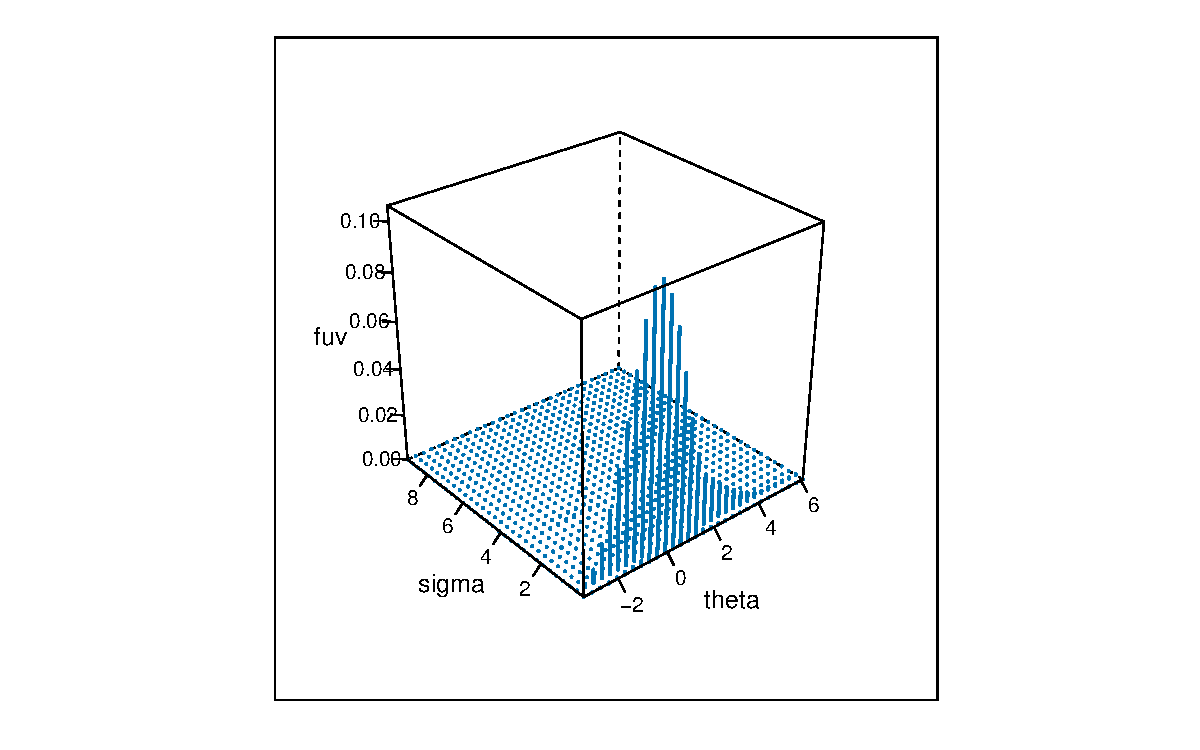
\includegraphics[width=\textwidth]{../../Figures/2013-2022/GMM_m/GLVmix_s.pdf}
    \end{figure}

    \column{0.5\textwidth}
    Case 2: $\sigma_i$ known.
    \begin{figure}
      \centering
      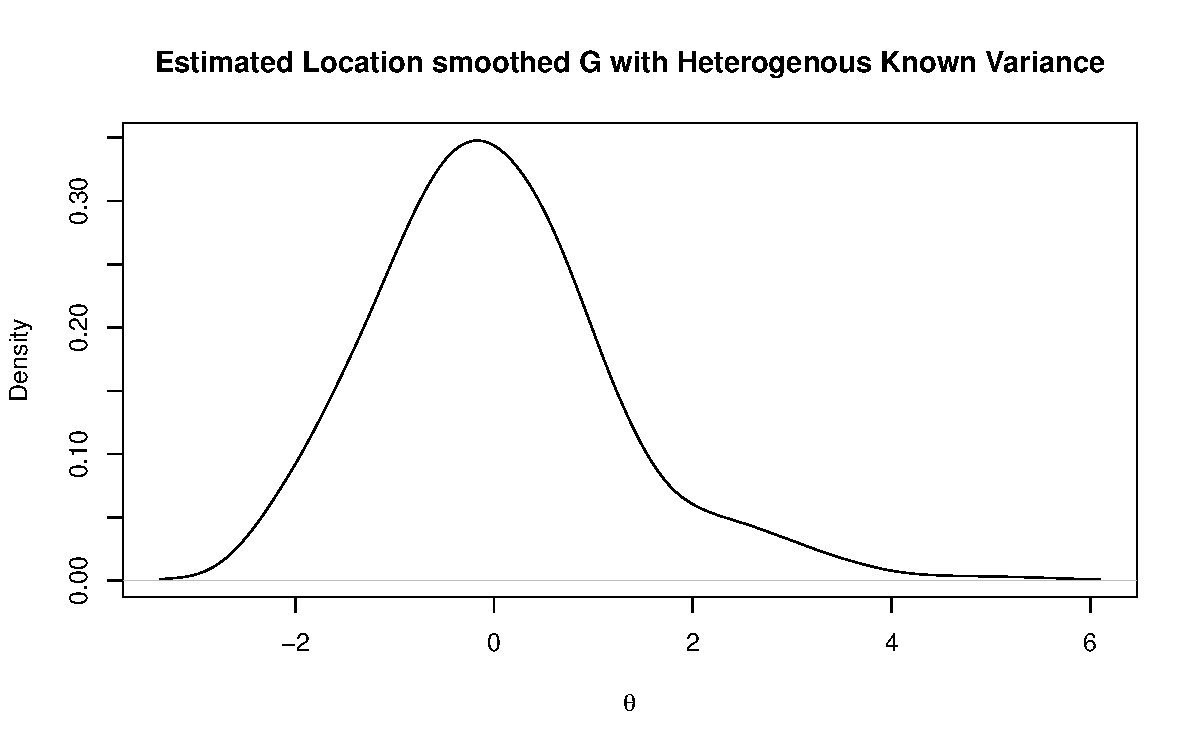
\includegraphics[width=0.9\textwidth]{../../Figures/2013-2022/GMM_m/GLmix_s.pdf}
    \end{figure}
  \end{columns}
\end{frame}

\begin{frame}
  \frametitle{Unknown $\sigma_i$: Posterior Tail probability}
  \begin{figure}
    \centering
    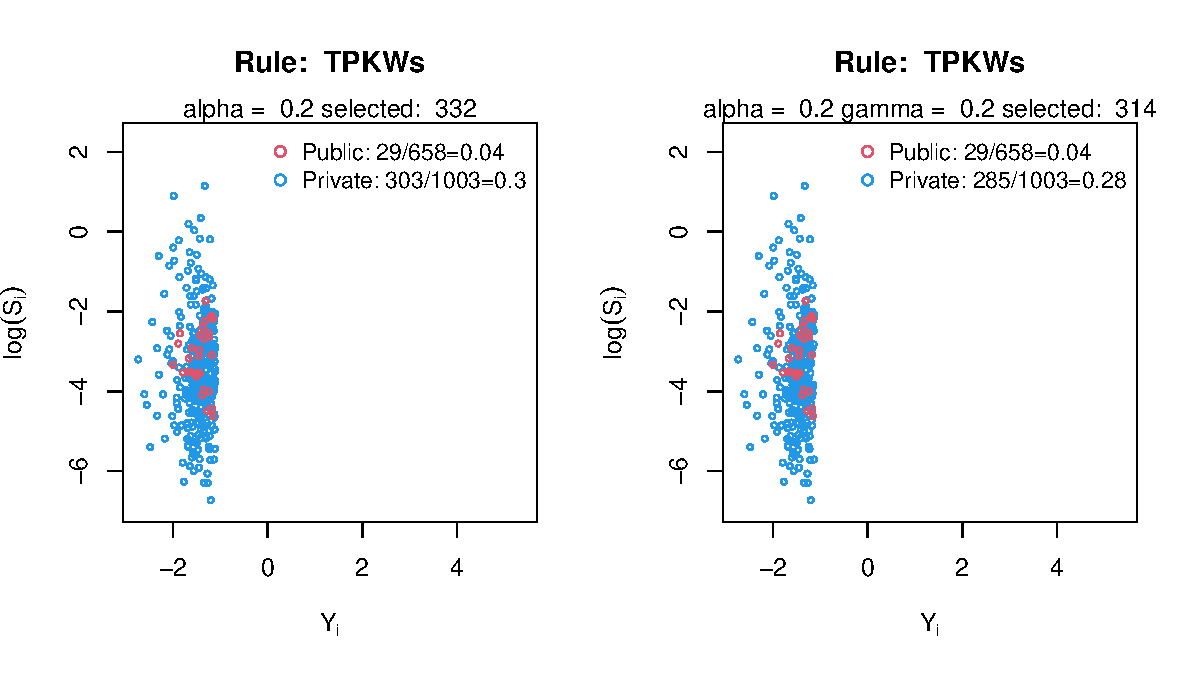
\includegraphics[width=0.9\textwidth]{../../Figures/2013-2022/GMM_m/GLVmix/Left_0.2_0.2_TPKWs.pdf}
  \end{figure}
\end{frame}

\begin{frame}
  \frametitle{Unknown $\sigma_i$: Posterior Mean}
  \begin{figure}
    \centering
    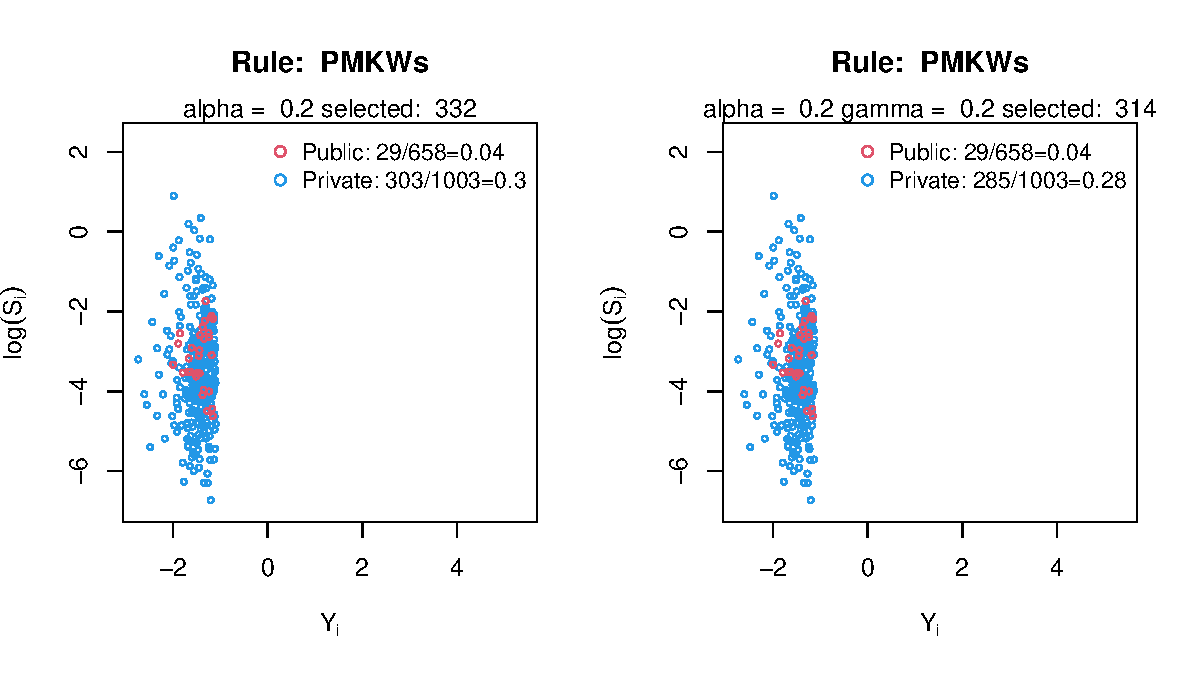
\includegraphics[width=0.9\textwidth]{../../Figures/2013-2022/GMM_m/GLVmix/Left_0.2_0.2_PMKWs.pdf}
  \end{figure}
\end{frame}

% \begin{frame}
%   \frametitle{Unknown$\sigma_i$: "Face value"}
%   \begin{figure}
%     \centering
%     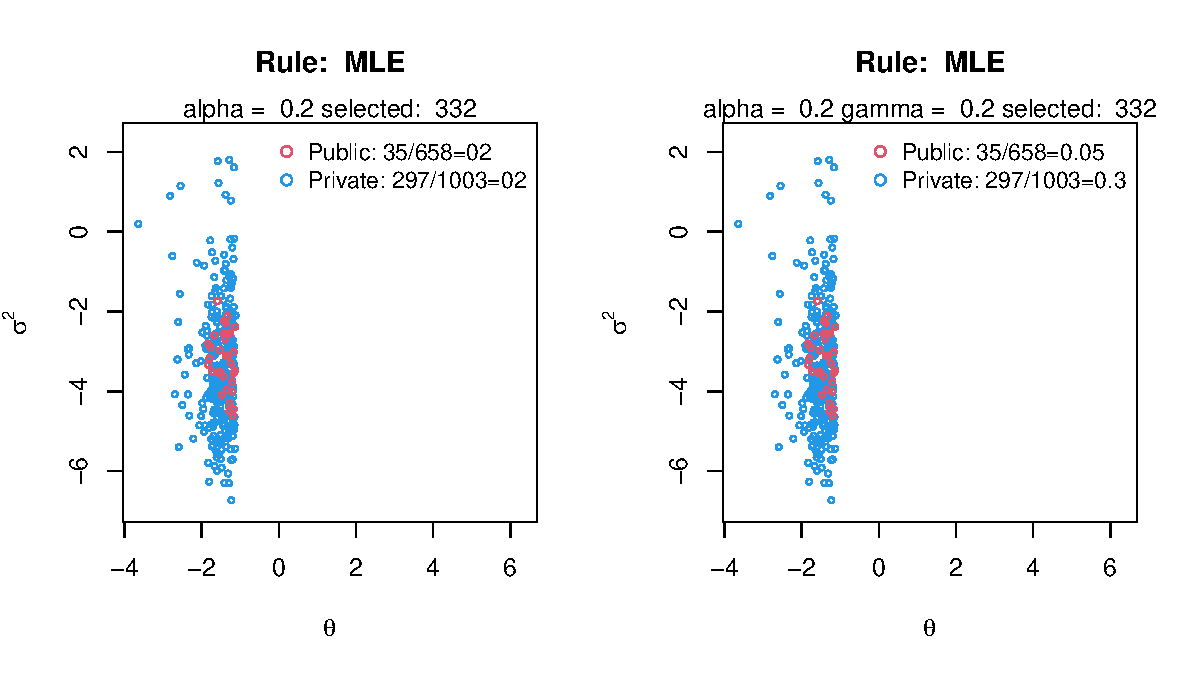
\includegraphics[width=0.9\textwidth]{../../Figures/2013-2022/GMM_m/GLVmix/Left_0.2_0.2_MLE.pdf}
%   \end{figure}
% \end{frame}

\begin{frame}[label=tpselect]
  \frametitle{Known $\sigma_i$: Posterior Tail probability}
  \begin{figure}
    \centering
    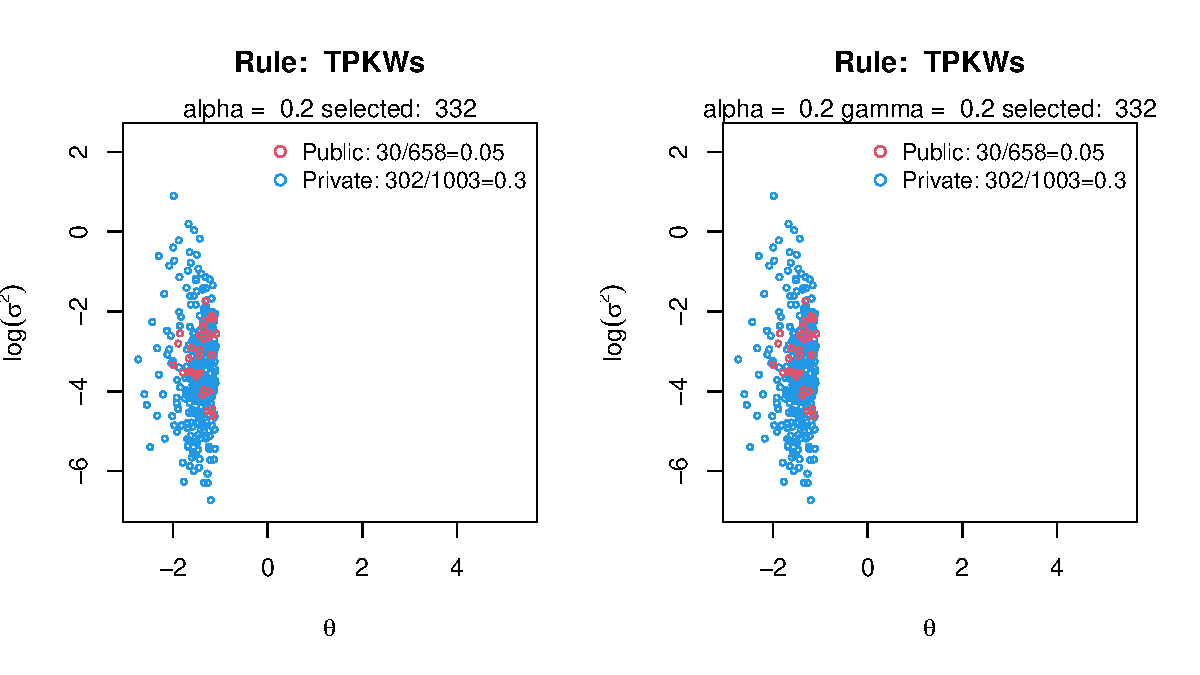
\includegraphics[width=0.9\textwidth]{../../Figures/2013-2022/GMM_m/GLmix/Left_0.2_0.2_TPKWs.pdf}
  \end{figure}
  \hyperlink{tpcontour}{\beamergotobutton{Next}}
\end{frame}

\begin{frame}
  \frametitle{Known $\sigma_i$: Posterior Mean}
  \begin{figure}
    \centering
    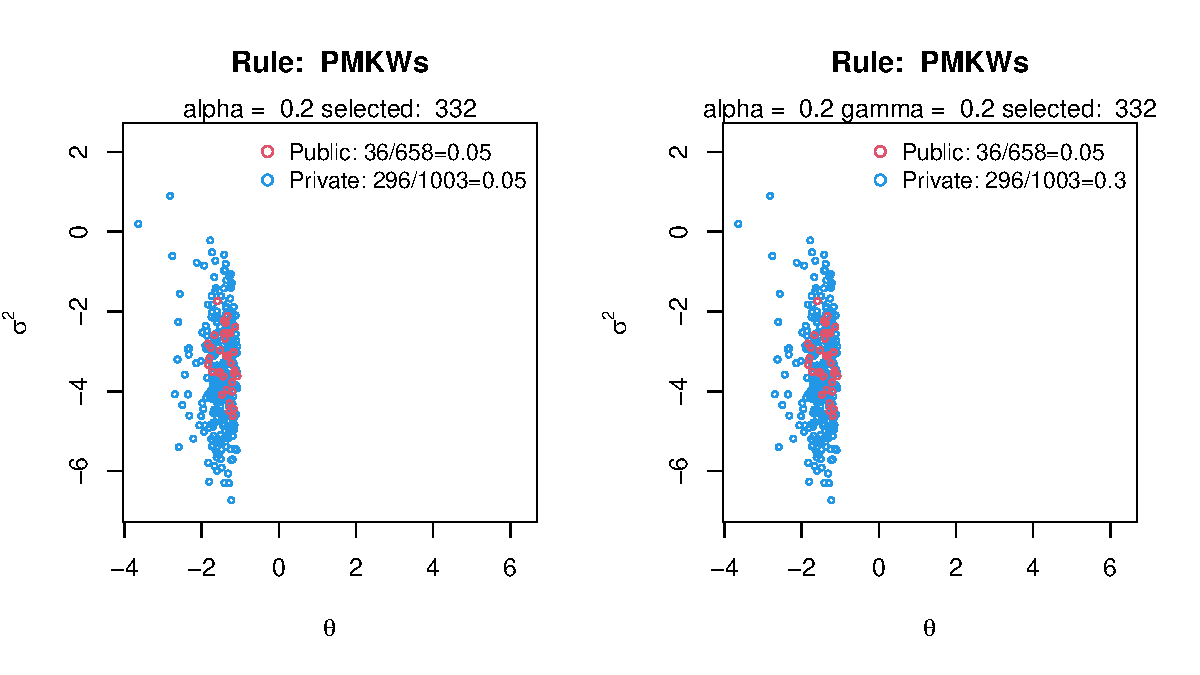
\includegraphics[width=0.9\textwidth]{../../Figures/2013-2022/GMM_m/GLmix/Left_0.2_0.2_PMKWs.pdf}
  \end{figure}
\end{frame}

\begin{frame}
  \frametitle{"Face value"}
  \begin{figure}
    \centering
    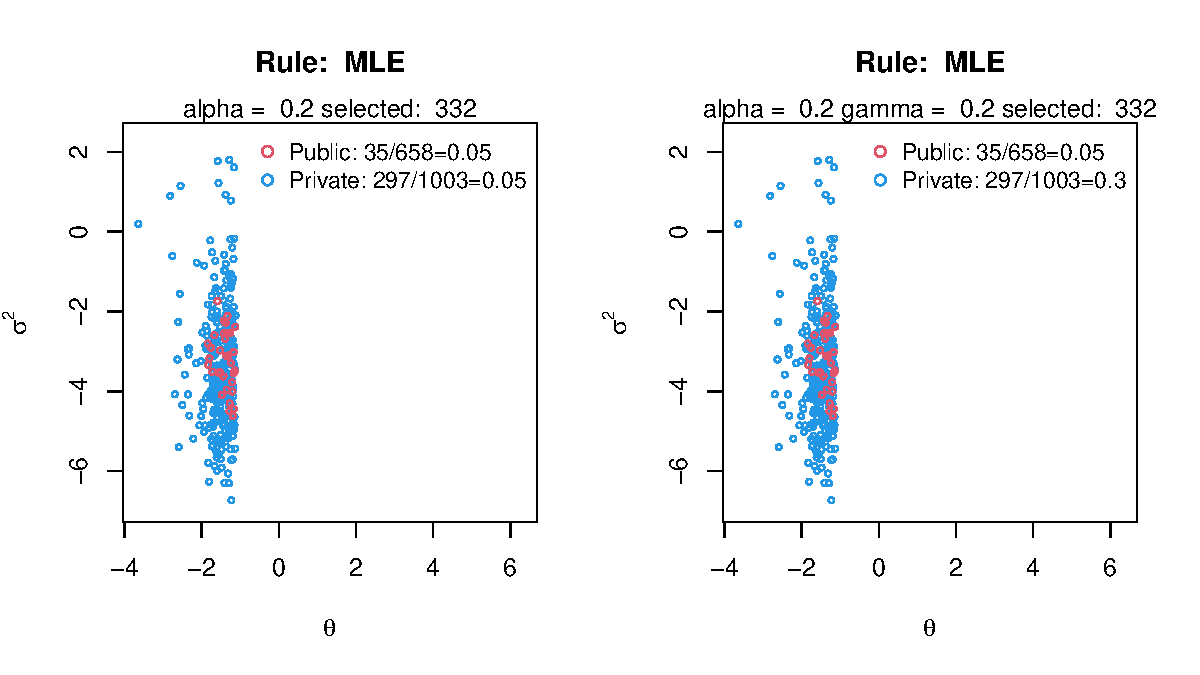
\includegraphics[width=0.9\textwidth]{../../Figures/2013-2022/GMM_m/GLmix/Left_0.2_0.2_MLE.pdf}
  \end{figure}
\end{frame}

\section{Conclusion}

\begin{frame}{Conclusion}
  \begin{itemize}
    \item Difference in whether to assume known $\sigma_i$.
    \item Control for the False Discovery Rate.
    \item Private (FP and NP) hospitals are indeed more "efficient".
  \end{itemize}
\end{frame}

\begin{frame}[label=limitation]{Limitation}
  \begin{itemize}\itemsep=12pt
    \item Interpretation of the $\theta_i$.
    \item Specification, endogeneity \textit{etc.}
    \item Normality assumption on $\varepsilon_{it}$.
          \hyperlink{normality}{\beamergotobutton{Next}}
  \end{itemize}
\end{frame}

\begin{frame}[allowframebreaks]
  \frametitle{References}
  \bibliography{../Thesis/ref.bib}
  \bibliographystyle{apalike}
\end{frame}

\appendix

\begin{frame}[label=normality]{Normality assumption on $\varepsilon_{it}$}
  Estimate the fixed effect $\theta_i$ by
  \begin{align*}
    \hat{\theta}_i =                       & \frac{1}{T}\sum(\theta_i+\varepsilon_{it}+x_{it}(\beta-\hat{\beta})) \\
    \overset{N\to \infty}{\longrightarrow} & \theta_i+\frac{1}{T}\sum_t \varepsilon_{it}
  \end{align*}
  When $T$ is relatively small (or even fixed), can't use central limit theorem to claim that $\hat{\theta}_i \overset{d}{\to} \caln(\theta_i,\frac{\sigma_i^2}{T})$.
  $\longrightarrow$ Assume that $\varepsilon_{it} \sim \caln(0,\sigma_i^2)$ .
  \hyperlink{observation}{\beamergotobutton{Back (main)}}   \hyperlink{limitation}{\beamergotobutton{Back (end)}}
\end{frame}

\begin{frame}[label=tpcontour]{TP vs PM}
  \begin{figure}
    \centering
    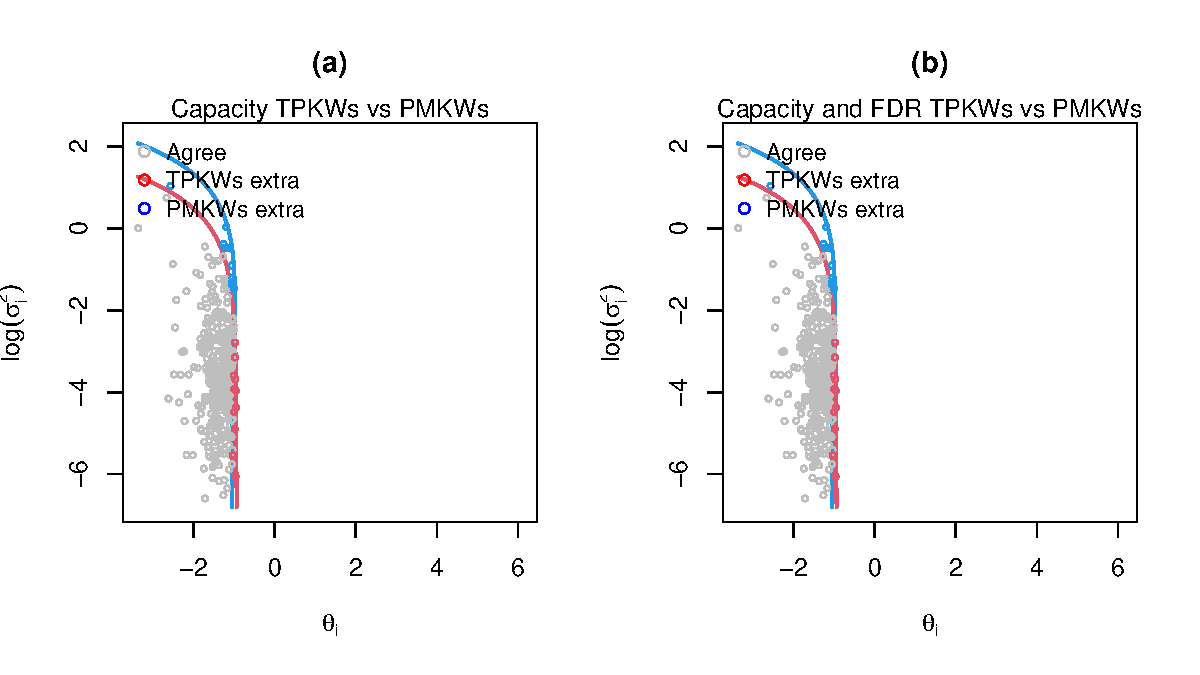
\includegraphics[width=0.9\textwidth]{../../Figures/2013-2022/GMM_m/GLmix/Contour_Left_0.2_0.2_TPKWs_PMKWs.pdf}
  \end{figure}
  \hyperlink{tpselect}{\beamergotobutton{Back}}
\end{frame}

\begin{frame}{TP vs JS}
  \begin{figure}
    \centering
    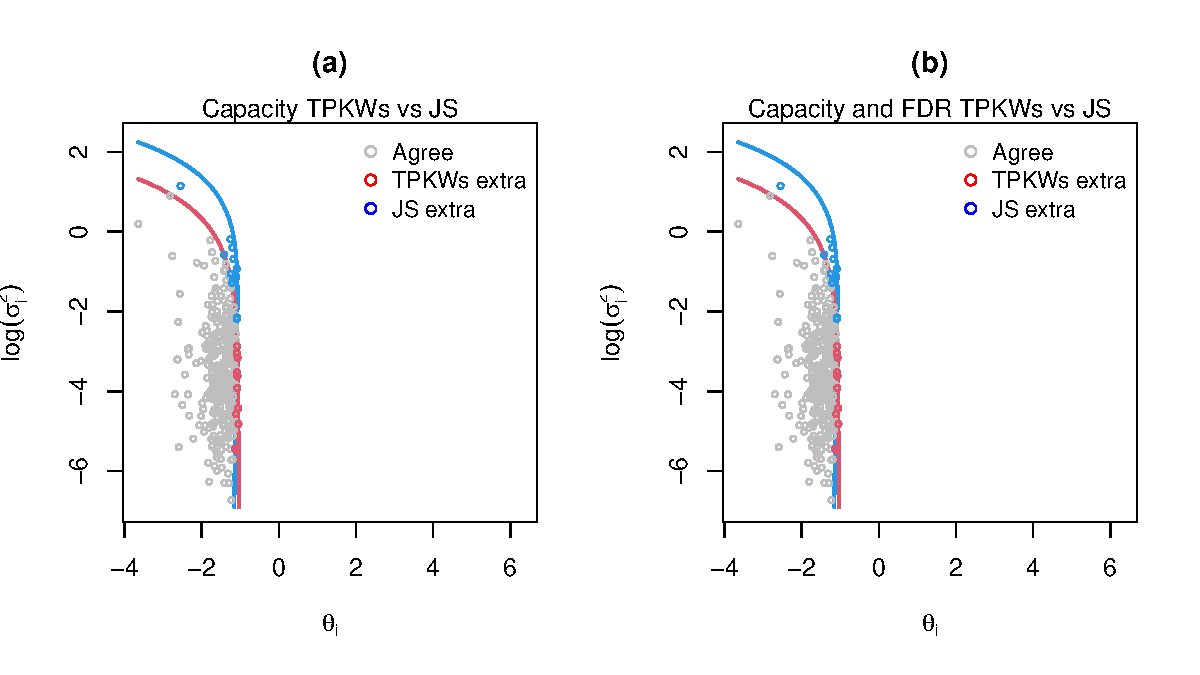
\includegraphics[width=0.9\textwidth]{../../Figures/2013-2022/GMM_m/GLmix/Contour_Left_0.2_0.2_TPKWs_JS.pdf}
  \end{figure}
\end{frame}

\begin{frame}{TP vs MLE}
  \begin{figure}
    \centering
    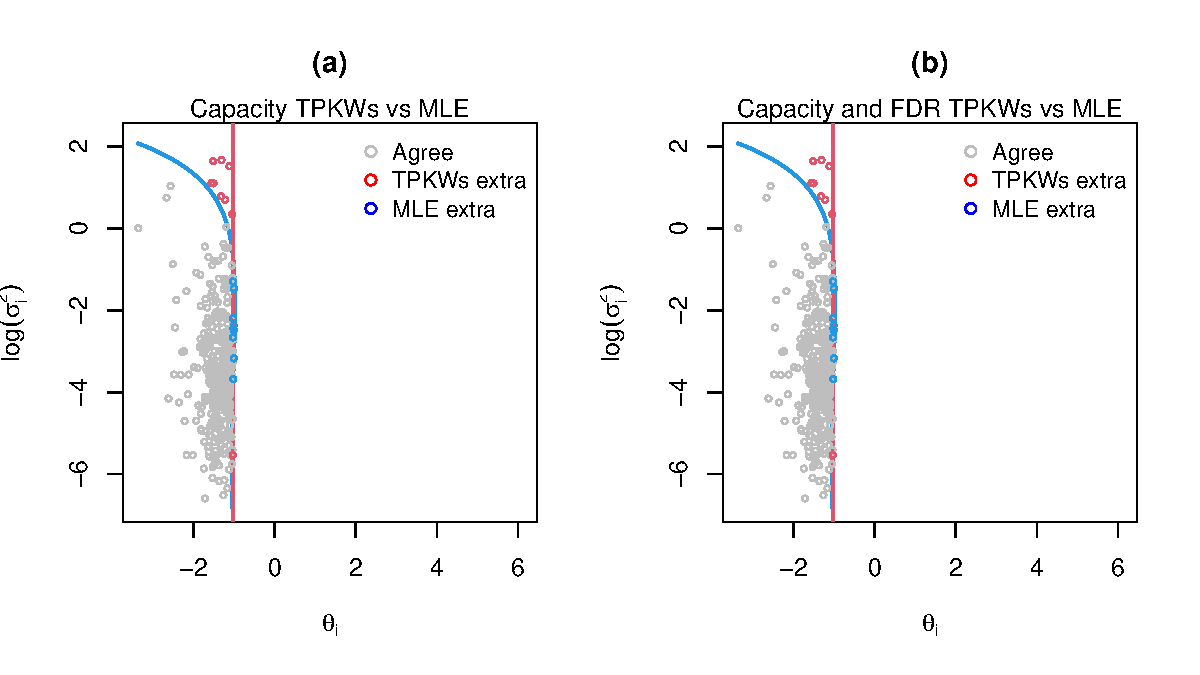
\includegraphics[width=0.9\textwidth]{../../Figures/2013-2022/GMM_m/GLmix/Contour_Left_0.2_0.2_TPKWs_MLE.pdf}
  \end{figure}
\end{frame}

\end{document}
